

\pagebreak 
\section{Matching Dynamics}
The baseline model of the search-and-matching labor market implicitly assumes free-entry for labor market firms, such that value of posting a vacancy is zero in equilibrium. This, in conjunction with linear vacancy posting costs, imply that the dynamic response of vacancies tend to be highly volatile and short lived. This is generally considered to be incompatible empirical responses of vacancies and unemployment rates, see for instance the general discussion in \citet{elsby2015beveridge}.


\subsection{Beveridge Curve}

Figure \ref{fig:Beveridge_cruve_data} shows the empirical Beveridge curve for the US 1951-2003. Conditioning on historical time periods the figure displays a clear negative correlation between the vacancy rate and the unemployment rate. In the context of search-and-matching models this is interpreted as the presence of pro-cyclical market tightness. That is, during an economic boom firms demand more labor through an increase in vacancy postings, but given decreasing returns to vacancies alone in the matching function firms must post an increasingly higher number of vacancies to increase their labor stock.\footnote{There is constant returns to the overall matching function so market tightness is not pro-cyclical if the numbers of searchers is sufficiently elastic. However, } This general a negative relationship between vacancy posting and the unemployment rate.




\begin{figure}[H]
\makebox[\linewidth][c]{%
\centering
  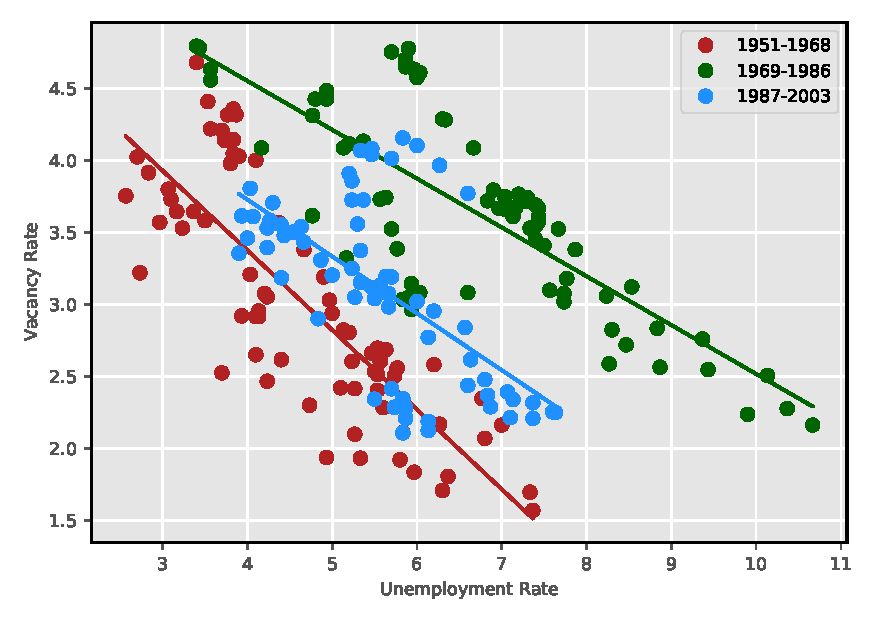
\includegraphics[width=.8\linewidth]{mainmatter/plots/Labor_market/Beveridge.pdf} 
}
\caption[Caption for LOF]{US Beveridge Curves 1951-2003}
\label{fig:Beveridge_cruve_data}
\centering
  {\scriptsize US Beveridge curve 1951-2003. The vacancy rate is proxied by the \textit{Composite Help-Wanted Index} from \citet{barnichon2010building}. The unemployment rate is obtained from FRED.  }
\end{figure}

\footnote{Since the model contains no aggregate shocks the Beveridge curve cannot be obtained through stochastic simulations. }

The empirical Beveridge curve is generated by a wide array of different shocks. In the theoretical framework presented earlier, I have primarily focused on a neutral technology shock.  


One way to generate non-jump dynamics of vacancies is to assume costly entry as in \citet{coles2018job}. A simpler way to generate more persistent dynamics in vacancy posting is to add quadratic costs to vacancy posting, contrary to the usual linear specification. Conjecturing that all firms choose the same amount of vacancies in equilibrium, the cost of posting vacancies is given by $\frac{\kappa_{V}}{2}V_{t}^{2}$. Labor demand obeys the same optimality condition as before:
\begin{gather*}
\mathcal{J}_{t}^{m}=\left(MPL_{t}-w_{t}h_{t}\right)+\frac{\left(1-\delta^{\text{L}}\right)}{1+r_{t+1}}\mathcal{J}_{t+1}^{m},,
\end{gather*}
where $\mathcal{J}_{t}^{m}$ measures the value of a match. Adding quadratic costs of vacancy posting affects only the optimal value of match, which is now given by $\mathcal{J}_{t}^{m}=\frac{\kappa_{V}V_{t}}{m_{t}}$, compared to $\mathcal{J}_{t}^{m}=\frac{\kappa_{V}}{m_{t}}$ from before.





To closer match the persistence observed in the data I follow \citet{fujita2007job} in modifying the vacancy creation process. 

Firms that want to enter the labor service sector must pay an additional cost $\kappa^{x}x_{t}$ where $x_t$ is the number of open positions in the economy at time $t$. The purpose of vacancies are to fill open positions. These can be open either because they have been created recently or because an existent match has been terminated through exogenous job destruction. Positions exist until they are terminated through obsolescence. 
Let $\delta^{O}$ denote the rate of job obsolescence. Let $\delta^{NO}$ denote the probability that a match is destroyed but the position not terminated. The job destruction rate that prevails at the aggregate level is given by $\delta^{N}=\delta^{O}+\left(1-\delta^{O}\right)\delta^{NO}$. That is, the sum of the probability that a job is destroyed by obsolesce $\delta^{O}$ and the probability that a match is destroyed given that the position is not made obsolete $\left(1-\delta^{O}\right)\delta^{NO}$. 

For households that are unemployed at time $t$ the probability of obsolescence imply that the Euler equation now reads:
\begin{gather*}
\left(c_{i,t}^{k=U}\right)^{-\frac{1}{\sigma}}=\beta\mathbb{E}_{i,t}R_{t+1}\left[\left(1-\delta^{O}\right)q_{t+1}\left(c_{i,t+1}^{k=N}\right)^{-\frac{1}{\sigma}}+\left(1-\left(1-\delta^{O}\right)q_{t+1}\right)\left(c_{i,t+1}^{k=U}\right)^{-\frac{1}{\sigma}}\right]
\end{gather*}
which reads that the households obtains employment with probability $q_t+1$ times the probability that the position is not made obsolete. The probability of remaining in unemployment is the complementary probability. Hence the new addition is that an unlucky share $\delta^{O}q_{t+1}$ of time $t$ searchers will find a job in the subsequent period, but this job will be made obsolete immediately. 
For employed households the Euler reads the same:
\begin{gather*}
\left(c_{i,t}^{k=N}\right)^{-\frac{1}{\sigma}}=\beta\mathbb{E}_{i,t}R_{t+1}\left[\left(1-\delta^{N}\left(1-q_{t+1}\right)\right)\left(c_{i,t+1}^{k=N}\right)^{-\frac{1}{\sigma}}+\delta^{N}\left(1-q_{t+1}\right)\left(c_{i,t+1}^{k=U}\right)^{-\frac{1}{\sigma}}\right]
\end{gather*}
though the job destruction rate $\delta^{N}$ has been redefined to include both destruction from obsolescence and from the termination of matches.  
The law of motion for employment reads:
\begin{gather*}
N_{t}=\left(1-\delta^{N}\right)N_{t-1}+S_{t}q_{t}\left(1-\delta^{O}\right),
\end{gather*}
which is only modified by the term $\left(1-\delta^{O}\right)$. 
Compared to the canonical search-and-matching model, where vacancies are a flow/jump variable, the above assumptions introduce a few additional dynamics for vacancies. Period $t$ vaccines $V_t$ is the sum of several flows: 
\begin{gather*}
V_{t}=\left(1-\delta^{O}\right)V_{t-1}+\left(1-\delta^{O}\right)\delta^{NO}N_{t-1}-\left(1-\delta^{O}\right)m_{t-1}V_{t-1}+x_{t}
\end{gather*}
taking them from left to right, the terms are: previous vacancies that have not been made obsolete $\left(1-\delta^{O}\right)V_{t-1}$, 
new vacancies that must be posted for positions that still exist but where the match has been terminated $\left(1-\delta^{O}\right)\delta^{NO}N_{t-1}$, vacant positions that were not made obsolete but were matched $\left(1-\delta^{O}\right)m_{t-1}V_{t-1}$ need not be filled again, the creation of $x_t$ new positions imply $x_t$ new vacancies must be posted. 

Given the redefinition of the job destruction rate the firms value of a match is unchanged:
\begin{gather*}
\mathcal{J}_{t}^{m}=\left(MPL_{t}-w_{t}\right)+\frac{\left(1-\delta^{N}\right)}{1+r_{t+1}}\mathcal{J}_{t+1}^{m},
\end{gather*}
Free entry imply that the value of a match must equal the cost $\mathcal{J}_{t}^{m}=\frac{\kappa_{V}V_{t}+\kappa_{x}x_{t}}{m_{t}}$. Since the cost posting vacancies and job openings affect the value of a match similarly they cannot both be identified from the steady-state. I hence set $\kappa_{V}=0$. 


\subsubsection{Calibration.} \citet{fujita2007job} finds that normal job destruction and obsoleting account for roughly and equal half of aggregate job destruction. I use this relation ship and set $\delta^{O}=\delta^{N}\frac{1}{2}$, where $\delta^{N}=0.06$ is the empirical estimate of the aggregate job destruction rate from XXX. The "normal" job destruction rate is then found residually as $\delta^{NO}=\frac{\delta^{N}-\delta^{O}}{1-\delta^{O}}$. The remaining calibration of the labor market is the same as earlier, though the calibrated job-finding rate changes slightly since the flow out of unemployment is affected by the job obsolesce rate. 